\documentclass[conference]{IEEEtran}

\usepackage{cite}
\usepackage{amsmath,amssymb,amsfonts}
\usepackage{algorithmic}
\usepackage{graphicx}
\usepackage{textcomp}
\usepackage{xcolor}
\usepackage{url}
\usepackage{flushend}

\def\BibTeX{{\rm
B\kern-.05em{\sc i\kern-.025em b}\kern-.08em
T\kern-.1667em\lower.7ex\hbox{E}\kern-.125emX}}

\begin{document}

\title{Detecting Harmful Medical Advice by Analyzing the
	Characteristics of Retweeters}

\author{\IEEEauthorblockN{Matthew Leon}
	\IEEEauthorblockA{\textit{Vanderbilt University}\\
		Nashville, Tennessee, USA\\
		matthew.leon@vanderbilt.edu}}

\maketitle

\begin{abstract}
	I study the ability of a model to discern, for tweets about the
	COVID-19 crisis and based on the characteristics of users who
	retweet it, whether or not a given article or tweet provides
	beneficial medical advice or could lead to a harmful outcome by
	promoting harmful medical practices or providing incomplete
	information that could lead to panicked action against the
	current medical wisdom. The model analyzes the characteristics
	of people who retweet the article, the pattern of how the
	article is retweeted, and what twitter uses say when retweeting
	the article.

	The study aims to support future work to identify and reduce
	the spread of panic-inducing misinformation and disinformation
	in an effort to help authorities better respond to
	health-threatening epidemics and pandemics.
\end{abstract}

\begin{IEEEkeywords}medical informatics, propagation, Twitter,
	medical advice, categorization, random forest, machine learning,
	social media, detection \end{IEEEkeywords}

\section{Introduction}

Online social media platforms from the likes of Facebook and
Instagram to the likes of Twitter all contain innumerable numbers
of fake profiles, troll accounts, and fake news posts, that lead
to a rapid spread of misinformation and disinformation. One of
the most consequential times for the spread of misinformation and
disinformation is in the middle of states of emergencies, and is
due to the lack of published, explicit responses from
governmental and/or authoritative sources to questions from the
public.  In these times, some social media users take to
publishing their own ``armchair expert'' opinions on social media
while others take to social media to find and solicit answers to
the questions they don’t have the information to answer. In these
circumstances, the ability for a computer to discern whether an
article represents sound advice is important: for one, the social
media platform itself can flag posts that appear suspicious in
order to curb the spread of misinformation while humans can
fact-check the information.

In the realm of biomedicine, the impact of disinformation becomes
even more important during times of medical crises. During the
2020 COVID-19 pandemic, the virus was not the only cause of
pandemic-related death: misinformation and misinterpretation of
legitimate information by officials of all levels led to the
death of at least one man, although many more are likely to have
been harmed by misinformation~\cite{fishtank}.

\section{Related Works}

Previous work by Aphinyanaphongs and Aliferis analyzed the
validity and trustworthiness of blog posts giving medical advice
for cancer treatments on the internet~\cite{textcat}. This work
utilized an analysis of the content of the article or blog post
to determine its authority based on the language used.  This work
is not directly applicable to information exchanged on social
media because the content of social media posts on Twitter, for
example, must be shorter than 280 (previously 140) characters.
This work could be used to analyze the actual article in
question, however. Later work by Liu Yang and Yi-Feng Brook Wu
during the 2016 US Presidential election season investigated the
effectiveness of modeling the propagation via shares of an
article for determining whether or not an article was ``fake
news''~\cite{fakenews}. Their findings opened up the possibility
for an article or blog post on Twitter to be classified as little
as five minutes after being posted based on the characteristics
of the people sharing the article as well as the pattern of
propagation, an idea also explored by Kwon, Cha, and
Jung~\cite{rumordetection}. The integration of multiple models
which categorize not just the temporal forces in propagation but
also the characteristics of the people retweeting a given article
allowed them to see much higher precision and recall in much less
time than previous efforts utilizing just one method or the
other.

Despite the apparent dangers of receiving information in
emergency situations from social media, Alexander found that
social media was used in seven different ways during crises: for
``listening to public debate, monitoring situations, extending
emergency response and management, crowd-sourcing and
collaborative development, creating social cohesion, furthering
causes (including charitable donation) and enhancing
research''~\cite{socialriskreduction}. Because there are a myriad
of benefits to social media, in addition to its necessity simply
because of prevalence, Alexander postulates that the
downsides---especially spreading of rumors and false
information---must be endured or dealt with, as ``the
incorporation of social media into pre-existing emergency
management systems is inevitable.'' This work shows that there
must be additional methods for curtailing rampant spread of
misinformation on social media in a way that does not hinder the
freedom of expression found on such networks.

\section{Hypothesis}

It is this researcher's goal to test the efficacy of existing
methods of detecting fake news and verify whether the existing
methodologies show promise in the detection of misinformation
stemming from the user characteristics of the tweets. In this
researcher's opinion, such work could be effectively implemented
a few different ways, each as a means to control the spread of
misinformation: for one, it could be a user-installed browser
extension which could be invoked to determine the reliability of
a tweet in question, or it could be implemented in the style of
stock market circuit breakers which pause trading on the stock
market to prevent panic~\cite{stockcircuitbreakers}. Such a
system could, when detecting patterns of unhelpful information,
alert relevant content moderators and pause sharing on the
article while its veracity is ascertained.

\section{Methods}

Tweets were collected from \textit{COVID-19: The First Public
	Coronavirus Twitter Dataset}~\cite{dataset}, and were downloaded,
cataloged and sorted as a preparatory stage of this project. The
initial focus was to find the the most popular
Coronavirus-related tweets on Twitter as measured by number of
retweets.  Next, the articles and source tweets were categorized
into three groups: ``helpful'', ``unhelpful'', and ``trash''.
Tweets which advocated, promoted, or explained helpful social
distancing measures, such as~\cite{goodolebarack}, were rated
``helpful''.  Tweets which advocated bad habits, such
as~\cite{dangeroustweeter}, were rated ``unhelpful''. This
category included tweets such as~\cite{sarcastictweet}, as in the
use case of a browser extension for users, a false negative
(resulting in believing harmful advice) is far more impactful
than a false positive (where the user would, on the
recommendation of the tool, not take the advice of a supposedly
sarcastic post). Tweets falling in the third category of
``trash'' were mostly related to album or movie releases, as
these tweets garner a large number of retweets and were included
in the COVID-19 dataset due to coronavirus hashtags written in
the comments.

The test and training sets were isolated from the top 300 tweets,
sorted by number of retweets. 71 tweets were thrown out as trash,
while 130 were rated ``unhelpful'' and 99 were rated ``helpful''.
The average user characteristics (listed at the end of the next
paragraph) for the first 40 retweets were added to each annotated
tweet. After this step, the tweets were filtered again to remove
any tweets for which the average user characteristics were
missing from the dataset (which is caused by the way Twitter's
Search API handles retweets without comments, which meant the
users were missing in the original dataset and is not
correctable without a professional subscription to Twitter's
API). The final total number of analyzed tweets included 69
marked as helpful and 87 marked as unhelpful, for a grand total
of 156 tweets.

A random forest was chosen for the classification, as it showed
better performance than a logistic regressive model also tested.
126 tweets were chosen for the training set, with 30 left for the
testing set (a 80/20 split).  The model was fed the average user
characteristic vector (containing 8 features) and a label, either
0 for so-called ``helpful'' tweets or 1 for an ``unhelpful''
tweet. Tweaking of the cost complexity pruning alpha of the
random forest resulted in a trained model that displayed
negligible signs of overfitting when the test and training sets
were compared, and further tweaking of the input user
characteristic vector showed that the most pertinent inputs were
the length of the user's description, the number of followers,
and the number of statuses posted by the user.  Additional input
features resulted in either equal or lower quality results. The
additional features tested included the length of the user's
screen name, the number of friends, the age of the user's
account, whether or not the account was verified, and whether the
user had changed the default profile information. The code used
to process the raw tweet data as well as the code to train the
model can be found at~\cite{myghrepo}.

\section{Results}

The final trained model displayed a total area under the ROC
curve of 0.755 for the test set, which is enough to discount
randomness, but not enough to use this model for a business
purpose. Using this model for the full set of data results in a
similar AUC of 0.720. The ROC curves are plotted for the full
set~(fig.~\ref{fullsetroc}) and the test
set~(fig.~\ref{testsetroc}).  The precision and recall are
detailed in table~\ref{precisionandrecall}.

\begin{table}[hb]
	\centering
	\begin{tabular}{rrrrr}
		  & Precision & Recall & F1-score & Support \\[6pt]
		0 & 0.60      & 0.69   & 0.64     & 13      \\
		1 & 0.73      & 0.65   & 0.69     & 17      \\[6pt]
	\end{tabular}
	\caption{Precision and Recall for model on test set}
	\label{precisionandrecall}
\end{table}

\begin{figure}[hb]
	\centering
	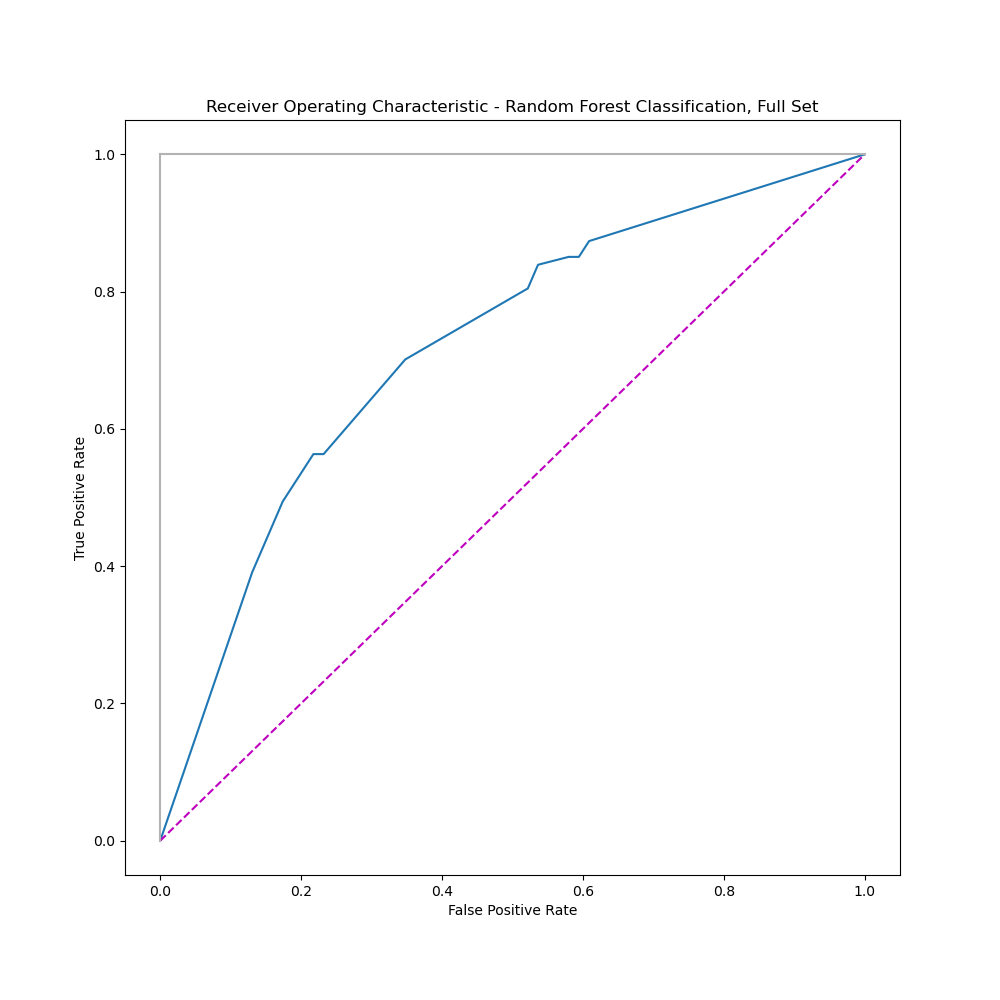
\includegraphics[width=0.5\textwidth]{full_set_auc.png}
	\caption{Full Set (Train \& Test) ROC}
	\label{fullsetroc}
\end{figure}

\begin{figure}[t]
	\centering
	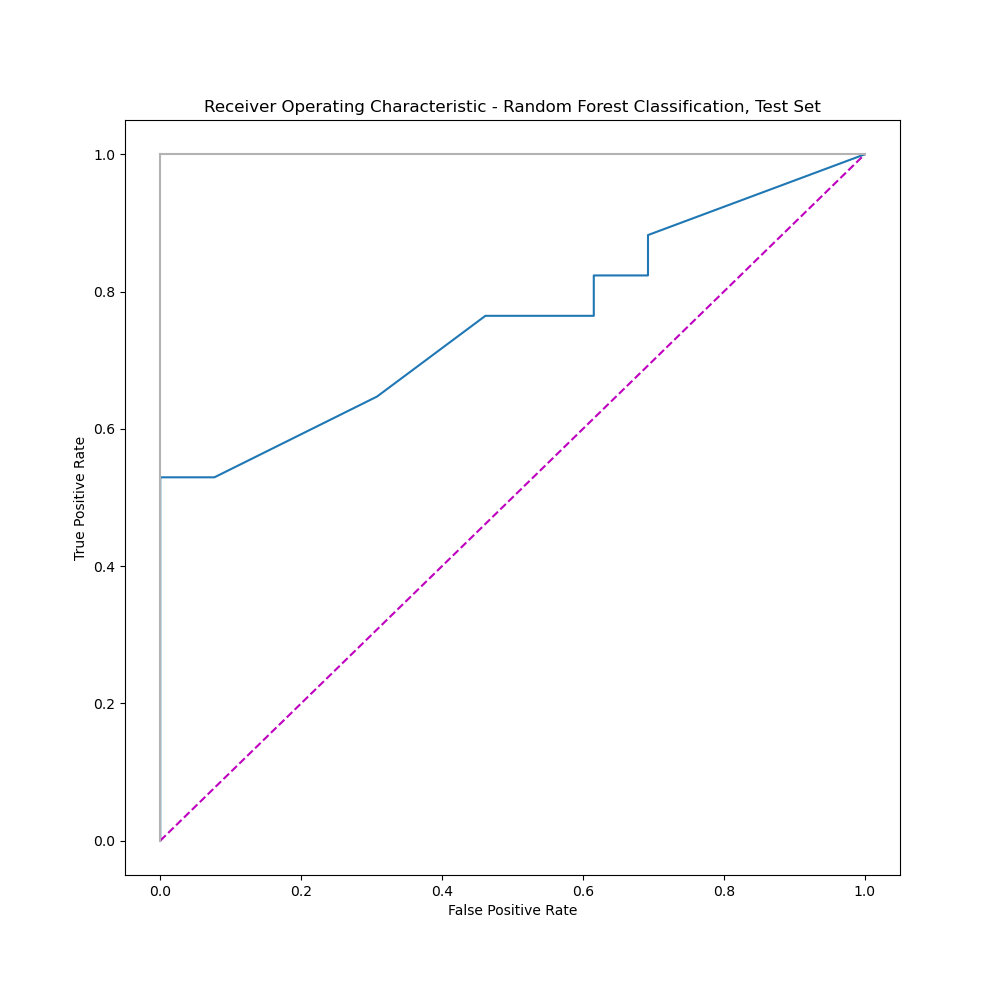
\includegraphics[width=0.5\textwidth]{test_set_auc.png}
	\caption{Test Set ROC}
	\label{testsetroc}
\end{figure}

\section{Analysis and Limitations}

There are several limitations with the data presented in this
study. For one, as was mentioned in the Methods section, the
dataset is missing retweets for certain tweets, corresponding to
those which were retweeted without any additional text. This is a
major limitation of the study, but can only be overcome with
access to the premium twitter API, as the tweets used in the
study were too old to use the free retweet lookup functionality
in the API.

Additionally, the only characteristics the end model used to
predict were the average retweeter's description length, number
of followers, and number of statues posted. These characteristics
are likely to bias the results in favor of established and
popular users on Twitter, becoming a rough measure of how much
``cred'' the users who retweet a post have; however, this is not
necessarily a bad thing as these accounts will often come from
relible news organizations and world thought leaders who
hopefully are more likely to fact-check before rampantly
retweeting. Such an assumption would require an entire study on
its own to confirm.

Adding additional measures to the model, such as combining the
results of the user characteristic measure with those from text
categorization of the post or article's content may prove to be
a more reliable measure; however, this comes with the difficulty
of parsing image and video content as well, as the researcher
anecdotes that several of the most helpful posts contained videos
of doctors or researchers breaking down complex topics about the
pandemic.

Additionally, the quality of this study and model can be thought
of more as a representation of how good a random forest can
predict whether Matthew Leon would find a given tweet ``helpful''
or ``unhelpful'', as the manual classifications contain his
personal biases towards certain content. Manual classifications
of only one non-expert source will certainly contain biases,
especially when much of the content rated contains partisan
political statements which have various shades of truth filtered
to suit political agendas rather straight helpful or unhelpful
medical advice. A more accurate model for determining the quality
of a tweet's medical advice may be made up of several layers: one
of which would detect whether or not a tweet contains political
content, another which would predict whether a tweet contains
advice or a command, and another to determine whether or not that
command is in-line with established practice, advises heeding the
advice of medical professionals, or spreads panic.
Unfortunately, this type of model would likely require training
on an established set of crisis-specific data available after the
crisis is complete, and may not be useful for emerging
situations. In such cases, a more generic model like that used in
this study, where the prediction is based upon factors other than
the content, may be more helpful.

Finally, this model was not tested in tweets that were unrelated
to the COVID-19 crisis, and thus testing such tweets may result
in highly erratic predictions.  This is an area of further
research to investigate the correlation between a tweet's content
and the characteristics of users who retweet it. The fact that
20\% of the top 300 tweets that were rated being labeled
``trash'' indicate that automated systems would need to have a
countermeasure to deal with this case.

\section{Conclusion}

This study set out to show that harmful medical advice could be
thwarted by a machine learning model tuned to characteristics
about users retweeting a given tweet. While definitive claims
applying the results may not be made, the results are indicative
of potential for more in-depth analysis factoring more features
into account.

\vspace{12pt}

\bibliographystyle{IEEEtran}
\bibliography{detecting-harmful-medical-advice-twitter}

\end{document}
